\section{Design}
\label{sec:design}

In this section, we describe the assumptions, design, and optimization of the protocol.

\subsection{Assumptions}

Our system design consists of three parties: Alice, Bob, and the aggregation server. In a typical application scenario, Alice may selectively publish her location datasets after encrypting them with her public key. Later, another user Bob queries on the location trajectories of Alice. The aggregation server is responsible to perform computation tasks on the encrypted data, and sends the (still encrypted) results to Alice. Alice is able to decide whether the query has intersection with the published data. If the query returns false, Alice is not able to learn about Bob’s location either.

We next describe what we mean by location datasets. Specifically, each user is able to represent their locations with GPS coordinates using tuples (latitude, longitude). One user may either specify a trajectory through consecutive tuples, or an area with tuple boundaries (e.g., a polygon or a circle). The goal of the aggregation server is that it is able to broadcast the encrypted location sets. To achieve this, each user also maintains a pair of public and private keys. Every bit of data, when sent to the server, will be encrypted using the public key to ensure security.

On the user side, we assume that Alice and Bob are usually not malicious. They will follow the protocol correctly but once the protocol has ended they can perform any computation they want on the information (encrypted or otherwise). If Alice finds out that there is an intersection with the trajectory of the query, the further interactions between Alice and Bob are out of scope of this protocol.


\subsection{Background}

We first describe the background of our work as follows.

\textbf{Homomorphic Cryptography:} Homomorphic encryption takes a foundational role in our system. Briefly, in fully homomorphic encryption~\cite{fan2012somewhat} and~\cite{van2010fully}, the following equations hold true:
\vspace{-0.1in}
\begin{equation}
m_1 + m_2 = D(E(m_1) + E(m_2))
\end{equation}
\begin{equation}
m_1 * m_2 = D(E(m_1) * E(m_2))
\end{equation}

In these equations, $E()$ stands for the encryption, $D()$ stands for the decryption. Computation can be done with encrypted values that translates to operations in the plain text domain. This allows parties to perform blind computation on encrypted values. In our design, we mostly rely on the addition operation rather than the multiplication operation due to the efficiency concerns.

\textbf{Bloom Filter:} We use standard notations on bloom filters to represent their operations, as follows:

\begin{itemize}
\item $m$: the total number of bits in the bloom filter;
\item $k$: the number of hash functions;
\item $n$: the number of elements inserted in the bloom filter;
\item $p$: false positive probability of the bloom filter;
\item $t$: the number of bits set to one.
\end{itemize}

The probability of false positives $p$ given a parameter set is:
\vspace{-0.1in}
\begin{equation}
p = (1-e^{\frac{-kn}{m}})^k
\label{equ:p}
\end{equation}

For a given $m$ and $n$, the value of $k$ that minimizes the false positive is:
\vspace{-0.1in}
\begin{equation}
k = \frac{m}{n}\ln2
\label{equ:k}
\end{equation}

For a given $n$ and the desired false positive $p$, the required number of bits $m$ is:
\vspace{-0.1in}
\begin{equation}
m = - \frac{n\ln p}{{(\ln2)}^2}
\label{equ:m}
\end{equation}


%For a given $m$, $k$ and $t$, the estimated elements in bloom filter is:

%\begin{equation}
%n* = - \frac{m\ln [1 - \frac{t}{m}]}{k}
%\label{equ:n}
%\end{equation}

We use these results later for performance analysis of our protocol.

\subsection{Main Protocol Idea with FHE}

The main idea for the protocol works as follows. The user Alice first inserts all locations as inputs to a configured bloom filter $BF$, by hashing locations to $k$ positions, and flipping corresponding bits. After all locations are inserted, suppose that this filter has $m$ bits, and $t$ bits have been set as $1$s, whose locations are specified as $b_1$,$b_2$,..., $b_t$. Our next goal is to encrypt the bloom filter $BF$ properly. Specifically, we observe that its set bits can be represented as a polynomial as:

\begin{equation}
\vspace{-0.1in}
f(x) = \prod_{i=1}^{t} (x-b_i)
\end{equation}

Alice then sends the encrypted polynomial $f(x)$ either in the product form or in the extended form to the aggregation server. Alice also sends the details on the $k$ hash functions, as well as the configuration parameters for the bloom filter. This is necessary as such information will later used by Bob for encryption needs as well. Even though A sends the hash functions, as the $f(x)$ is encrypted with the public key, the aggregation server has no way to learn which bits have been set as $1$ in the bloom filter.

The aggregation server next waits for the query from Bob. However, Bob does not send the query, i.e., locations, in plain text either. Instead, Bob will first obtain the $k$ hash functions from the server, and hash the query locations into $k$ bits as $p_1$, $p_2$, $\cdots$, $p_k$. Bob would like to test if all these bits have been set as $1$ in the encrypted bloom filter sent by Alice. To do this, Bob sends the $k$ positions to the server, which then can calculate for each location, whether the polynomial has a corresponding bit set as $1$. To do this, we can test each of the $k$ positions individually, by evaluating of $f(x)$ in the encrypted form as $E(f(p_i))$. We know that, based on the nature of this encryption method, the following equation also holds true:

\begin{equation}
\vspace{-0.1in}
D(E(f(p_i))) = f(p_i)
\end{equation}

Furthermore, if $p_i$ has been flipped to $1$ by Alice earlier, this evaluation result must be $0$ based on the product nature of the polynomial. Therefore, if we construct another polynomial as $\sum_{i=1}^{k}(E(f(p_i)^2)$ (we use square is to prevent the evaluation may sometimes lead to negative numbers), we have:

\begin{equation}
\vspace{-0.1in}
H(p) = D[\sum_{i=1}^{k}(E(f(p_i))^2] = \sum_{i=1}^{k}(f(p_i)^2)
\end{equation}

Observe that in this equation, only when all $k$ bit locations have been flipped to $1$, the result $H(p)$ will be $0$. If $H(p)$ is not $0$, then it means that the query is not in the bloom filter. We note that the multiplication steps for computing $H(p)$ is $t$ (based on the factorized form of $f(x))$, the total time of multiplication involved is $O(k*t)$. A large $t$, like 200, makes such a multiplication impractical for two reasons: first, the fast growth of ``inherent noise'' in ciphertexts of FHE schemes makes them likely to be corrupted very quickly, which limits the computation capacity greatly; second, the fast increased size of ciphertexts worsens the computation overhead. Some techniques, such as relinearization~\cite{brakerski2012leveled} and approximate eigenvector method~\cite{gentry2013homomorphic}, have been proposed to balance the multiplication computation capacity and computation overhead, but they still do not work efficiently on a huge multiplication depth in real applications. So, we design the following alternative protocols containing limited or no multiplication operations. We call these protocols \emph{practical} for this reason.




\subsection{Practical Protocol 1: An Improved Implementation of the Homomorphic Bloom Filter}
\label{subsec:basic_implementation}

We now describe the first working implementation using fewer additions and multiplications compared to the primitive idea above. Its pseudocode is shown in Algorithm \ref{alg1}. Alice first inserts her locations into a bloom filter $BF$ using $k$ hash functions, where $t$ bits have been set as $1$, and the corresponding positions are specified as $b_1, b_2, \dots, b_t$. Then Alice uses her public key $PK$ to encrypt each negated $b_i$ as the encrypted $E(-b_i)$, which are then submitted to the aggregation server. After launching a query, Bob first asks the public key $PK$ and the same $k$ hash functions from Alice. Then Bob hashes his query location into k bits as $p_1, p_2, \dots, p_k$, which are then encrypted as $E(p_1), E(p_2), \dots, E(p_k)$ by $PK$ and submitted to the same aggregation server. Once receiving the encrypted query from Bob, the server starts the evaluation based on $E(b)$ and $E(p)$. Specifically, for each $E(p_j)$, the server performs $E(p_j) + E(-b_i)$, where $i = 1, 2, \dots, t$, and gets $t$ encrypted results which are then decrypted as $D(E(p_j) + E(-b_i))$ respectively by Alice using her secret key $SK$. Notice that in this design, the information of Bob might still be leaked to Alice no matter whether they have trajectory intersections or not, because Alice can obtain the value of $p_j$ by:
\begin{equation}
p_j =\frac{\sum_{i = 1}^{t}[D(E(p_j) + E(-b_i)) + b_i]}{t}
\end{equation}

To address this problem, we introduce the randomness during the evaluation by multiplying $E(p_j) + E(-b_i)$ by a random positive integer $z$. Thus, if $D(E(p_j) + E(-b_i))$ equals 0, $D((E(p_j) + E(-b_i))*z)$ still equals 0, while other values vary dramatically. Once one of the $t$ encrypted results of $p_j$ equals 0, it means the position of $p_j$ in $BF$ is set as 1. If all positions of $p_j$ for $j$ from $1$ to $k$ in $BF$ is set as 1, we can conclude Bob has an interaction with Alice with a certain confidence level which are determined by $BF$'s rate of false positives (we analyze the impact of this false positive rate later). Otherwise, Bob has no intersection with Alice at the query location $100\%$.


\begin{algorithm}\small
\caption{A Basic Implementation of the Homomorphic Bloom Filter}
\label{alg1}
\begin{algorithmic}[1]

\Statex Alice: Bloom Filter Encryption
\State $b \gets BF.get\_ones\_positions()$
\For{$i = 1 \to t$}
    \State $E(-b_i) \gets$ encrypt $-b_i$ using $PK$
\EndFor
\State send $E(-b)$ to the aggregation server

\item[]

\Statex Bob: Query Encryption
\State $p \gets$ hashed value of his location
\For{$j = 1 \to k$}
    \State $E(p_j) \gets$ encrypt $p_j$ using $PK$
\EndFor
\State send $E(p)$ to the aggregation server

\item[]

\Statex Sever: Evaluation
\For{$j = 1 \to k$}
    \For{$i = 1 \to t$}
        \State $cipher\_result_{ij} \gets (E(p_j) + E(-b_i))*z$
    \EndFor
\EndFor
\State send $cipher\_result$ to Alice

\item[]

\Statex Alice: Result Decryption
\For{$j = 1 \to k$}
    \State $flag \gets FALSE$
    \For{$i = 1 \to t$}
        \State $plain\_result_{ij} \gets$ decrypt $cipher\_result_{ij}$ using $SK$
        \If {$plain\_result_{ij} = 0$}
            \State $flag \gets TRUE$
            \State \textbf{break}
        \EndIf
    \EndFor
    \If {$flag = FALSE$}
        \State \textbf{return} no intersection
    \EndIf
\EndFor
\State \textbf{return} intersection exists

\end{algorithmic}
\end{algorithm}



\subsection{Practical Protocol 2: A Lightweight Evaluating Implementation of the Homomorphic Bloom Filter}
The previous protocol requires $k*t$ additions and one-depth multiplications respectively for evaluation and $k*t$ times of decryptions in the worst case, which may pose a burden on the speed of query. In this section, we propose an improvement that requires $k$ additions, no multiplication and one decryption to speedup the query. The pseudocode is shown in Algorithm \ref{alg2}. Like protocol 1, Bob queries Alice's locations. After inserting her locations into the bloom filter $BF$, Alice encrypts every bit, $b_1, b_2, \dots, b_m$, in $BF$ and submits $E(b)$ to the aggregation server. Then Bob uses the same $k$ hash functions Alice uses to hash his query location into $p_1, p_2, \dots, p_k$ which actually are the corresponding bit positions in $BF$. These hashed values $p$ are submitted to the server in plaintext, which we think is still safe because the chosen $k$ cryptohash functions ensure that the server cannot reversely compute the plain text from hashed values. The server then sums all elements in $E(b)$ whose index is in $p$. Then the server subtracts $k$, i.e., the length of $p$, from the sum and returns the cyphertext result to Alice for decryption. The whole evaluation and decryption can be expressed as follows:

\begin{equation}
plain\_result = D(\sum_{j = 1}^{k}E(b_{p_j}) - E(k))
\end{equation}

If $plain\_result$ equals 0, it implies that all values of $b_{p_j}$ are same and equal 1. In other words, all positions of $p_j$ in $BF$ are flipped as 1. So, we can say Bob interacts Alice with a certain probability of false positive expressed by Equation \ref{equ:p}. Otherwise, they do not intersect at the query location 100\%.

\begin{algorithm}\small
\caption{A Lightweight Evaluating Implementation of the Homomorphic Bloom Filter}
\label{alg2}
\begin{algorithmic}[1]


\Statex Alice: Bloom Filter Encryption
\State $b \gets BF.get\_all\_elements()$
\For{$i = 1 \to m$} \Comment{$m$ is the size of $BF$}
    \State $E(b_i) \gets$ encrypt $b_i$ using $PK$
\EndFor
\State send $E(b)$ to the aggregation server

\item[]

\Statex Bob: Query Encryption
\State $p \gets$ hashed value of his location
\State $E(k) \gets$ encrypt $k$ using $PK$
\State send $E(k)$ and $p$ to the aggregation server

\item[]

\Statex Sever: Evaluation
\State $sum \gets 0$
\For{$j = 1 \to k$}
    \State $sum \gets sum + E(b_{p_j})$
\EndFor
\State $cipher\_result \gets sum - E(k)$
\State send $cipher\_result$ to Alice

\item[]

\Statex Alice: Result Decryption
\State $plain\_result \gets$ decrypt $cipher\_result$ using $SK$

\end{algorithmic}
\end{algorithm}


\subsection{Practical Protocol 3: A Bit-wise Implementation of the Homomorphic Bloom Filter}

\begin{figure}[t]
    \centering
    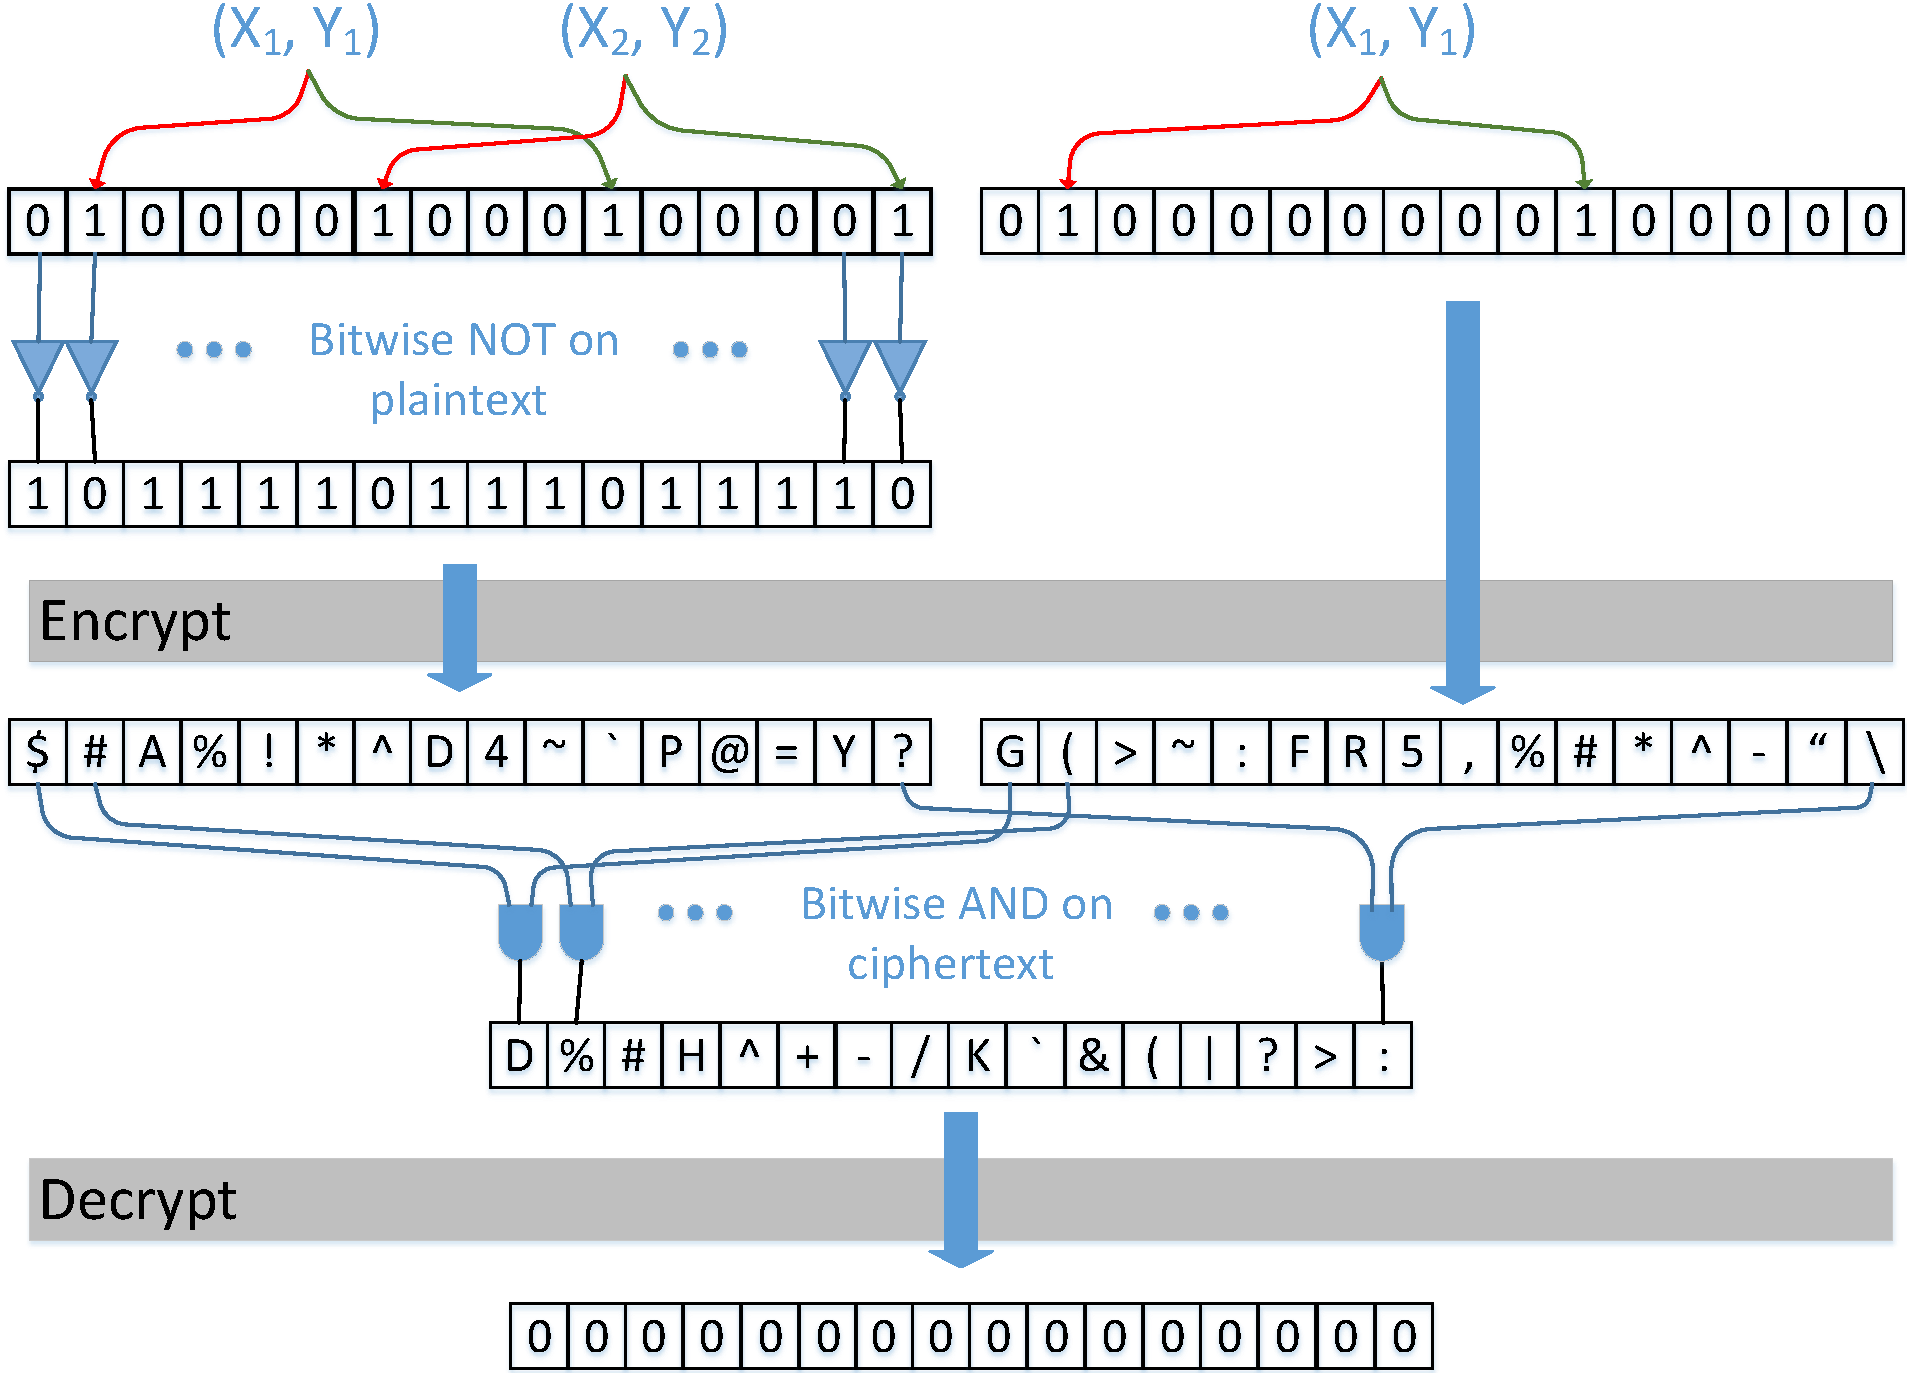
\includegraphics[width=0.8\linewidth]{figures/bitwise_bloomfilter.pdf}
    %\vspace{-0.1in}
    \caption{Bloom filter encrypted query with bitwise encryption scheme}
    \label{fig:bloomfilter_bitwise}
    \vspace{-0.1in}
\end{figure}

Although the previous design was feasible, it is built entirely on top of the underlying homomorphic encryption scheme, and treats such a scheme as a blackbox. The advantage of doing this is that even if we change the implementation of the homomorphic encryption, this design does not need to be modified.

However, we also observe that the recently proposed homomorphic encryption schemes are usually based on bit-wise operations, a feature that is highly similar to the underlying scheme of bloom filters. This similarity lends itself to cross-layer optimization, where we demonstrate that it is possible to directly leverage the lower-level implementations to speed up our design algorithm. Specifically, modern homomorphic encryption methods encrypt data in a bit-wise manner, i.e., each bit in the plaintext is encrypted as a separate ciphertext. Later, the computation is represented as a boolean circuit with XOR and AND gates, where the input is the ciphertext for each encrypted bit. As this mechanism breaks down an arbitrary computation into bit operations, this may lead to highly complex circuits. However, after transforming the original query operation that involved several arithmetic operations into the query operation based on bloom filter, the query operation can be more easily decomposed to bit-wise operations.

Recall that the underlying data structure of bloom filter is a bit array with length of that can be naturally represented as an array of integers, which is precisely the required input for homomorphic encryption systems. As the homomorphic encryption method encrypt each bit of the integer, it actually encrypts each bit of bloom filter into a ciphertext. Therefore, we naturally obtain the encrypted bloom filter without using the polynomial method as developed in the previous section.

Specifically, we re-design the query operation as follows. Observe that based on bloom filter, the query operation can be decomposed as bit-wise operations as following. Suppose Alice uses her data to construct a bloom filter $BF_A$ with all her locations inserted into  this filter. Bob also constructs a bloom filter $BF_B$ with only the location he wants to query.  To check whether the location that Bob wants to query is in Alice’s location set, one only need to check if all bits that are set in $BF_B$ are also set in $BF_A$. To check this, first one can use bit-wise AND operation to get a bit array containing wanted bits in $BF_A$. Then it is sufficient for us to check whether all wanted bits are set, where one can simply perform a bit-wise XOR operation with the resulting bit array from last step. Therefore, the query operation can be decomposed into two bit-wise operation as following:

\begin{equation}
\vspace{-0.1in}
BF_{A} \& BF_{B} \oplus BF_{B}
\label{math:band}
\end{equation}

If the query returns positive result, i.e., the queried location of Bob is exist in Alice’s location set, we know that the value of \autoref{math:band} is zero.

Furthermore, the operation can be simplified as:

\begin{equation}
\vspace{-0.1in}
\neg BF_{A} \& BF_{B}
\label{math:band_simple}
\end{equation}

Here, the bit-wise NOT operation only requires one input, thus can be performed locally before the encryption occurs. This can further reduce the required operation overhead under encryption form.

With \autoref{equ:m}, we can calculate the optimal $m$ given a certain number of elements $n$ and required false positive level $p$. We use $l$ to represent the length of an integer. Then the system needs to encrypt $\lceil m/l \rceil$ integers. During query, the system needs to calculate encrypted AND operation for $\lceil m/l \rceil * l$ bit. In the last step, the system needs to decrypt $\lceil m/l \rceil$ integers to get the result. Before the computation, both the Alice and Bob need to send their bloom filter to the server which is $\lceil m/l \rceil$ integers. After the computation has been done, $\lceil m/l \rceil$ integers need to be send back as the result.


\subsection{Geohash-based Homomorphic Bloom Filter}
To further improve the scalability and reduce the transmission overhead of the homomorphic bloom filter, our next optimization handles how to encode location datasets, especially areas, effectively. We adopt a method called the Geohash~\cite{moussalli2015fast}, which is a base-32 geocoding system, and can convert any coordinate pair into a short alphanumeric string of which each character is written in base-32. The precision of Geohash conversion can be adjusted by the length of the alphanumeric string. Each Geohash covers one rectangular region within which all coordinate pairs share this Geohash as their common prefixs. For example, the Geohash \textbf{dp3t} in Figure \ref{fig:geohash} represents the rectangular area with red boundary lines, which could be divided into 32 sub-regions by appending one extra character. Note that all the sub-regions, such as \textbf{dp3t0}, \textbf{dp3tz}, share \textbf{dp3t} as the longest common prefix. Normally, a longer common shared prefix means a shorter distance between the these locations. Besides, the sub-region identified by \textbf{dp3t0} can also be divided into 32 sub-sub-region by appending an additional character recursively.

\begin{figure}
    \centering %dp3t
    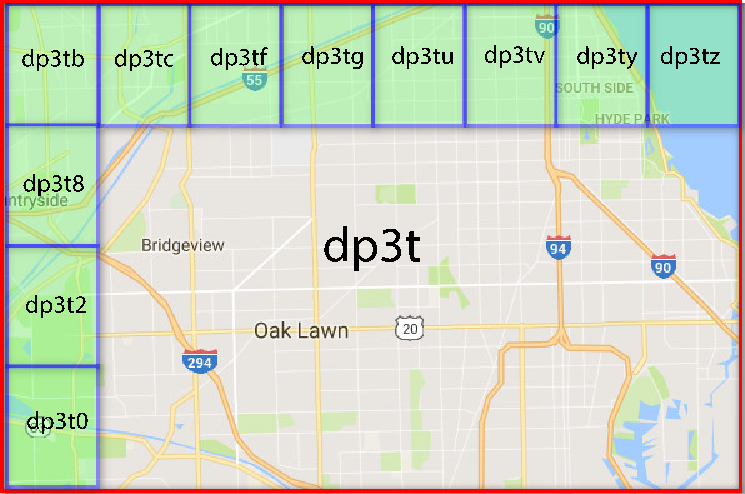
\includegraphics[width=0.35\textwidth]{./figures/geohash.pdf}
    \caption{Geohash method overview}\label{fig:geohash}\vspace{-0.1in}
\end{figure}

Our idea is that only the locations in a certain region represented by one Geohash can be inserted into an identical bloom filter labeled by this Geohash, i.e., any locations outside this region are never allowed to inserted into this bloom filter. Possible largest areas (the areas decrease from the equator to the poles) covered by different Geohash lengths are illustrated in Table \ref{tab:geohash_region_size}. Because the region size of the Geohash length of 4 is so large, the bloom filter size has to be very large to contain all possible locations in this region, and the region size of the Geohash length of 6 is so small that it is easy to guess users' locations once the Geohash becomes available. So, normally we take the Geohash length of 5 to identify a bloom filter, i.e., all the locations within a certain region of 4.89km x 4.89km are inserted into a bloom filter. Note that the optimal Geohash length might depends on the environment. For example, a shorter Geohash length probably works very well in the desert areas or at sea, but on Manhattan Island a longer length can be used safely.

\begin{table}[]
\centering
\footnotesize
\caption{Metric Dimensions of the Region Covered by Different Geohash Lengths}
\label{tab:geohash_region_size}
\begin{tabular}{|c|c|c|}
\hline
Geohash Length & Region Width & Region Height \\
\hline
1 & 5,000km & 5,000km \\
2 & 1,250km & 625km \\
3 & 156km & 156km \\
4 & 9.1km & 19.5km \\
5 & 4.89km & 4.89km \\
6 & 1.22km & 0.61km \\
7 & 153m & 153m \\
8 & 38.2m & 19.1m \\
9 & 4.77m & 4.77m \\
10 & 1.19m & 0.596m \\
11 & 149mm & 149mm \\
12 & 37.2mm & 18.6mm \\
\hline
\end{tabular}
\normalsize
\vspace{-0.1in}
\end{table}

Suppose Bob queries the location of Alice. With the Geohash-based homomorphic bloom filter, Alice sends all her encrypted Geohash $E(G_a)$ to the aggregation server. Bob also submits his encrypted Geohash $E(G_b)$ to the server. Then the server checks whether the $G_b$ is in $G_a$ or not, by subtracting $E(G_b)$ from each element in $E(G_a)$, and sends the ciphertext results to Alice for decryption. Once Alice finds out no plaintext result equals 0, we can conclude that there is no intersection between Alice and Bob. Otherwise, Alice can identify the bloom filter $BF$ where Bob's location may exist by:


\begin{equation}
BF = \frac{\sum_{i = 1}^{s}G_{ai} - \sum_{i = 1}^{s}D(E(G_{ai}) - E(G_b))}{s}
\label{math:hash_lable}
\end{equation}




where $s$ is the size of $G_a$. Then all the protocols we mentioned before can be used for a further query.




